\documentclass[main.tex]{subfiles}
\begin{document}

\section*{Sheet 2}

\subsection{Exercise 1}

The motion of a photon in Schwarzschild spacetime can be described, 
assuming without of generality it lies in the \(\theta = \pi / 2\) plane, 
by the normalization of its 4-velocity %
\begin{align} \label{eq:photon-velocity-normalization}
0 = u^2 = - \left(1 - \frac{2M}{r}\right) \dot{t}^2 + \left(1 - \frac{2M}{r}\right)^{-1} \dot{r}^2 + r^2 \dot{\varphi}^2
\,,
\end{align}
%
where dots denote derivatives with respect to an affine parameter \(\lambda\). 

We can use two Killing vectors of this spacetime, \(\partial_t\) and \(\partial_\varphi\), 
to compute integrals of motion: %
\begin{align}
e &= - u \cdot \partial_t = \left(1 - \frac{2M}{r}\right) \dot{t}  \\
l &= u \cdot \partial_\varphi = r^2 \dot{\varphi}
\,.
\end{align}

These are conserved across the photon's motion, therefore it is convenient to use them to 
eliminate the functions \(t(\lambda )\) and \(\varphi (\lambda )\) in equation \eqref{eq:photon-velocity-normalization}, 
so that we get a differential equation for \(r(\lambda )\) only, parametrized by \(e\) and \(l\).

The computation goes as follows; let us denote \(A =1 - 2M/r\) for brevity: 
%
\begin{align}
0 &= - A \left( \frac{e}{A}\right)^2 + \frac{\dot{r}^2}{A} + r^2 \left( \frac{l}{r^2}\right)^2   \\
0 &= - \frac{e^2}{A} + \frac{\dot{r}^2}{A} + \frac{l^2}{r^2}  \\
e^2 &= \dot{r}^2 + \frac{l^2}{r^2} A \\
\underbrace{\frac{\dot{r}^2}{2}}_{\text{kinetic}} 
\underbrace{+ \frac{l^2}{2r^2} - \frac{l^2M}{r^3}}_{\text{potential}} &= \underbrace{\frac{e^2}{2}}_{\text{total}} \label{eq:photon-trajectory-schwarzschild}
\,.
\end{align}

We found something in the form of an energy conservation equation, 
with a kinetic term \(\dot{r}^2 / 2\) and an effective potential. 

For large \(r\) the potential will approach 0 from above, like \(1/r^2\), 
while for small \(r\) it will approach negative infinity like \(- 1/ r^3\).
Therefore, it will have a maximum, which is easily computed to lie at \(r = 3M\). 
There, the value of the potential \(V _{\text{eff}}\) is 
%
\begin{align}
l^2 \left( \frac{1}{2 (3M)^2} - \frac{M}{(3M)^3}\right) 
= \frac{l^2}{M^2} \left( \frac{1}{18} - \frac{1}{27} \right) = \frac{l^2}{54M^2}
\,.
\end{align}
%

For photons starting at \(\mathscr{I}^-\), 
this potential barrier might be insurmountable depending on \(M\), \(l\) and \(e\): 
the condition to check for insourmountability is whether 
%
\begin{align}
\frac{e^2}{2} < \frac{l^2}{54 M^2}
\,,
\end{align}
%
which means %
\begin{align}
\frac{l^2}{e^2} > 27M^2
\,.
\end{align}

What is the physical meaning of the ratio \(l/e\)?
it can be shown to correspond 
(up to a \(\pm\) sign, which depends on whether the motion is clockwise or counterclockwise) 
to the impact parameter \(b\), 
the distance between the asymptotic trajectory of the photon and the 
center of the black hole. 
The proof goes as follows: 
%
\begin{align}
\frac{l}{e} \approx r^2 \frac{\dot{\varphi}}{\dot{t}} = r^2 \dv{\varphi}{t}
\,,
\end{align}
%
where we used the fact that \(e = (1-2M/r) \dot{t} \approx \dot{t}\) at radial infinity; then, 
\begin{align}
\dv{\varphi}{t} = \dv{\varphi}{r} \underbrace{\dv{r}{t}}_{\approx -1 } = 
- \dv{r} \arcsin (b / r) \approx - \dv{r} ( \pm b/r) = \mp \frac{b}{r^2}
\,,
\end{align}
%
therefore \(l/e = \mp b\) --- the linear order approximation is justified since
we are only interested in the asymptotic behaviour.

Therefore, photons with an impact parameter \(b\) larger than \(\sqrt{27} M \approx 5.2M\)
will not be able to surmount the potential barrier and "bounce off" it, 
going back to radial infinity, while the ones with smaller \(b\) 
will cross the potential barrier, moving further towards the horizon and then the singularity.

The \(b = \sqrt{27}M\) case is degenerate, as it describes three distinct trajectories: 
photons approaching from \(\mathscr{I}^-\), which spiral forever, 
asymptotically approaching \(r = 3M\); photons stuck in an unstable 
orbit at \(r = 3M\); and finally photons which reach the singularity at
some finite time after having orbited since past infinity. 

\subsection{Exercise 2}

We discuss negative-mass Schwarzschild spacetime, and define a radial coordinate %
\begin{align}
\rho = r + 2M \log (1 - r / 2M) = r - 2 \abs{M} \log (1 + r / 2 \abs{M})
\,.
\end{align}

The \(r \to \infty \) limit corresponds to \(\rho \to \infty\); 
at \(r = -2M\) we have \(\rho = -2M(1 - \log 2) \approx - 0.6 M\) (\(>0\)), 
and finally for \(r \to 0^+\) we get \(\rho \to 0^+\). 
Thus, the range of \(\rho\) is \((0, + \infty )\) just like \(r\)'s, 
although their relation is nonlinear. 

The differential of \(\rho\) will read %
\begin{align}
\dd{\rho } &= \pdv{\rho }{r} \dd{r} = \left( 1 + \frac{2M}{1 - r / 2M} \left(- 2M\right)\right) \dd{r}  \\
&= \left( 1 - \frac{2M}{2M - r} \right) \dd{r} = - \frac{r \dd{r}}{2M - r}
\,,
\end{align}
%
therefore %
\begin{align}
\dd{\rho}^2 = \left(\frac{r}{r-2M}\right)^2 \dd{r}^2 = \left(\frac{r}{r + 2 \abs{M}}\right)^2 \dd{r}^2
\,.
\end{align}

The metric will read as follows, in terms of \(\rho\) (and denoting \(r = r(\rho )\)): 
%
\begin{align}
\dd{s^2} &= - \left( 1 - \frac{2M}{r}\right) \dd{t^2} + \frac{1}{(1 - 2M/r) (r/(r-2M))^2} \dd{\rho^2} 
+ r^2 \dd{\Omega^2}  \\
&= - \left( 1 - \frac{2M}{r}\right) \dd{t^2} + \left( 1 - \frac{2M}{r}\right) \dd{\rho^2} 
+ r^2 \dd{\Omega^2}  \\
&= \underbrace{\left(1 + \frac{2 \abs{M}}{r} \right)}_{>0} \left(- \dd{t}^2 + \dd{\rho }^2\right) + r^2 \dd{\Omega}^2
\,.
\end{align}

We can see that the \((t, \rho)\) section of the metric is conformally related 
to flat spacetime, since the prefactor in front of it is always positive. 

The angular section is not the same as the one of the corresponding flat spacetime, 
since the prefactor in front of it is 
%
\begin{align}
\frac{r^2}{1 - 2M/r} \neq \rho^2
\,,
\end{align}
%
but this only means that we cannot interpret \(\rho\) as the radius defined 
by the area of a sphere: \(\rho \neq \sqrt{A / 4 \pi }\).

The conformal diagram for this spacetime will therefore look the same as Minkowski, 
with the caveat that the prefactor diverges for \(r \to 0\): so, the 
\(r = 0 \) line will not be a reflective boundary in this case. 
Indeed, just like in positive-mass Schwarzschild the Kretschmann scalar diverges there, 
so it is a singularity.

However, there are no horizons --- this spacetime is conformally related to Minkowski which has no horizons; 
alternatively, we can see that the whole spacetime is in the causal past of future null infinity.
This means that the singularity is naked!

\subsection{Exercise 4}

(I switched the order since this exercise is related to exercise 2)

The trajectories in negative mass Schwarzschild can be computed in the same manner as in positive mass Schwarzschild, the difference will be in the asymptotics of the potential. 
For photons we have the same result as in equation \eqref{eq:photon-trajectory-schwarzschild}: the effective potential is %
\begin{align}
V _{\text{phot}} = l^2 \left( \frac{1}{2r^2} - \frac{M}{r^3}\right)
\,,
\end{align}
%
and a total ``energy'' of \(E = e^2 /2\),
while for massive particles the same calculation, but with \(u^2 = -1\), yields 
%
\begin{align}
V _{\text{mass}} = - \frac{M}{r} + l^2 \left( \frac{1}{2r^2} - \frac{M}{r^3}\right)
\,,
\end{align}
%
but now the total ``energy'' is \(E = (e^2- 1) / 2\).

In both cases, the equation of motion reads %
\begin{align}
\frac{\dot{r}^2}{2} + V = E
\,.
\end{align}

This holds for positive and negative-mass Schwarzschild alike, since no assumptions are made about the sign of \(M\). 
However, the asymptotics will change depending on its sign. 

In the photon case, the potential will read 
%
\begin{align}
V _{\text{phot}} = l^2 \left( \frac{1}{2r^2} + \frac{\abs{M}}{r^3}\right)
\,,
\end{align}
%
which is monotonic (it's the sum of two monotonic terms) and strictly positive, as long as \(l \neq 0\). 
It approaches 0 at \(r \to + \infty \) like \(l^2 / 2 r^2\), just like the positive-mass case, but as \(r \to 0^+\) it goes like \(l^2 \abs{M} / r^3 \to + \infty\). 

So, any photon with nonzero \(l\) will not be able to reach the singularity, since it will have a finite \(e\) (recall from exercise 1 that the impact parameter is \(l / e\)). 

On the other hand, photons with \(l = 0\) exactly will move according to \(\dot{r}^2 = e^2 = \text{const}\). 
This means that they will reach the singularity \(r = 0\) in a finite amount of time, and their trajectories cannot be extended beyond this point: the spacetime is null geodesically incomplete. 

For massive particles, the potential looks like 
%
\begin{align}
V _{\text{mass}} = + \frac{\abs{M}}{r} + \frac{l^2}{2 r^2} + \frac{l^2 \abs{M}}{r^3}
\,,
\end{align}
%
which is fully repulsive, regardess of whether the angular momentum is vanishing or not! 

This might be expected: we are looking at a negative-mass object, the effect of gravity is reversed. 
This potential approaches 0 like \(1 / r\) for \(r \to +\infty \), and it approaches \(+ \infty \) like \(1 / r^3\) for \(r \to 0^+\) if the angular momentum is nonzero, like \(1/ r\) if the angular momentum is zero. 

Any timelike geodesic will have a finite \(E\), therefore at some radius it will invert: specifically, when \(E = \abs{M} / r\), we must have \(\dot{r} = 0\), and the trajectory going back away from the black hole.

This means that no timelike trajectory can actually approach \(r = 0\), they all can be extended arbitrarily: the spacetime is timelike geodesically complete! 

This feature is hard to represent in a conformal diagram, since it is spefically about the properties of timelike geodesics, which are not faithfully rendered in such diagrams.

\subsection{Exercise 3}

The conformal diagram for Minkowski spacetime is constructed by setting 
%
\begin{align}
t - r &= u = \tan U  \\
t + r &= v = \tan V
\,,
\end{align}
%
transforming the non-angular section of the metric as 
%
\begin{align}
\dd{s^2} &= - \dd{t^2} + \dd{r^2}  \\
&= - \dd{u} \dd{v}  \\
&= \frac{- \dd{U} \dd{V}}{(\cos U \cos V)^2}
\,,
\end{align}
%
and relating this to the new metric \(\dd{\widetilde{s}}^2 = - \dd{U} \dd{V}\), which has the same null geodesics as \(\dd{s}^2\) since they are conformally related. 

The ranges of these new coordinates are \(U, V \in (- \pi /2, \pi /2)\), 
and \(V \geq U\); the \(V = U\) line corresponds to \(r = 0\). 

All relevant trajectories are shown in figure \ref{fig:conformal_trajectory}. 

\begin{figure}[ht]
\centering
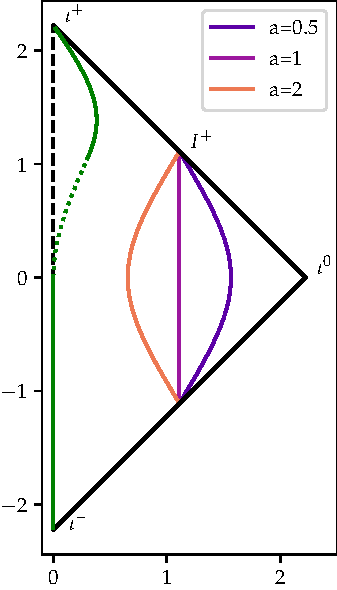
\includegraphics[width=.35\textwidth]{figures/conformal_trajectory}
\caption{Conformal diagram for the trajectories parametrized by \(\lambda \), as well as (in green) a trajectory starting off at \(r = 0\), accelerating (dotted), then moving geodesically from then on.}
\label{fig:conformal_trajectory}
\end{figure}

Our second trajectory is parametrized as \(t = \sinh(a \lambda ) / a\) and \(r = \cosh(a \lambda ) / a\) 
for some real number \(a\).

This means that %
\begin{align}
U &= \arctan(t-r) = \arctan(\frac{\sinh(a \lambda ) - \cosh(a \lambda )}{a})  \\
V &= \arctan(t+r) = \arctan(\frac{\sinh(a \lambda ) + \cosh(a \lambda )}{a})
\,.
\end{align}

Now, we have the following identities: %
\begin{align}
\sinh x - \cosh x &= \frac{e^x - e^{-x}}{2} - \frac{e^x + e^{-x}}{2} = - e^{-x}  \\
\sinh x + \cosh x &= \frac{e^x - e^{-x}}{2} + \frac{e^x + e^{-x}}{2} = e^{x}  
\,.
\end{align}

Therefore, %
\begin{align}
U &= \arctan(- \frac{e^{-a \lambda }}{a}) \\
V &= \arctan(\frac{e^{a \lambda }}{a})
\,.
\end{align}

Now, \(\arctan(-x) = - \arctan{x}\), and also \(\arctan(1 / x) = \pi /2 - \arctan{x}\). 

This means that, for example, if \(a = 1\) we get 
%
\begin{align}
U + V = \pi / 2
\,,
\end{align}
%
a straight line going from a point in \(\mathscr{I}^{-}\) to a point 
in \(\mathscr{I^{+}}\). 

If \(a \neq 1\) the line is not straight, but its endpoints are the same ones. 

This curve is timelike: its tangent vector is \(u = (\cosh(a \lambda ), \sinh(a \lambda ), 0, 0)\), whose modulus is 
%
\begin{align}
u^2 = - \cosh^2(a \lambda ) + \sinh^2(a \lambda ) = -1 
\,.
\end{align}

The proper time is computed as 
%
\begin{align}
\tau = \int \frac{ \dd{t}}{\gamma }
\,,
\end{align}
%
where \(\gamma = 1/ \sqrt{1 - v^2}\), \(v\) being the coordinate velocity:
what is it? 
%
\begin{align}
v = \dv{x}{t} = \dv{\cosh(a \lambda )}{\sinh(a \lambda )} = \dv{\sqrt{T^2 + 1}}{T} = \frac{T}{\sqrt{T^2 + 1}} = \frac{\sinh(a \lambda )}{\cosh(a \lambda )} = \frac{t}{x} 
\,,
\end{align}
%
where \(T = a t = \sinh(a \lambda )\); therefore 
%
\begin{align}
\frac{1}{\gamma } = \sqrt{1 - \frac{T^2}{T^2 +1}} = \sqrt{\frac{T^2 +1 - T^2}{T^2 + 1}} = \frac{1}{\sqrt{T^2 + 1}}
\,,
\end{align}
%
meaning that 
%
\begin{align}
\tau = \int \frac{ \dd{T}/a}{\sqrt{T^2 +1}} = \frac{1}{a}\operatorname{arcsinh}
(T) = \lambda 
\,.
\end{align}

The proper acceleration is then easily computed: the proper-time derivative of the velocity is \(\dv*{u}{\tau } = A = (a \sinh(a \lambda ), a \cosh(a \lambda ), 0, 0) \), so 
%
\begin{align}
A^2 = - a^2 \sinh(a \lambda ) + a^2 \cosh(a \lambda ) = a^2
\,.
\end{align}

Thus, \(a\) is the (constant) proper acceleration of this curve, and \(\lambda = \tau \) is its proper time parameter.

Now: how can this timelike curve start and end at \(\mathscr{I}^{\pm}\)? 
It's accelerating forever, so it asymptotes to lightlike

\todo[inline]{say this better}

\subsection{Exercise 5}

The Kerr metric in Boyer-Lindquist coordinates reads %
\begin{align}
\mathrm{d}s^2 = - \frac{\Delta}{\rho^2} 
\left(\mathrm{d}t^2 - a \sin^2 \theta \mathrm{d}\varphi \right)^2
+ \frac{\sin^2 \theta}{\rho^2}
\left( (r^2 + a^2) \mathrm{d}\varphi - a \mathrm{d}t\right)^2
+ \frac{\rho^2}{\Delta } \mathrm{d}r^2 + \rho^2 \mathrm{d}\theta^2
\,,
\end{align}
%
where \(\Delta = r^2 - 2Mr + a^2\) and \(\rho = r^2 + a^2 \cos \theta \).

We have the Killing vectors \(\partial_t\) and \(\partial_\varphi \), which determine two integrals of motion of the trajectory we can associate with energy and angular momentum respectively. 

The angle \(\theta\) is measured from the ``north pole'', so the equatorial plane corresponds to \(\theta = \pi / 2\). Since \(\dot{\theta} = 0\) initially, this will hold for the whole trajectory (by the \(\theta \to \pi - \theta \), \(\varphi \to - \varphi \) symmetry of the metric): therefore, we can use the reduced equatorial metric %
\begin{align}
\mathrm{d}s^2 &= - \frac{\Delta}{\rho^2} 
\left(\mathrm{d}t^2 - a \mathrm{d}\varphi \right)^2
+ \frac{1}{\rho^2}
\left( \rho^2 \mathrm{d}\varphi - a \mathrm{d}t\right)^2
+ \frac{\rho^2}{\Delta } \mathrm{d}r^2   \\
&= 
- \frac{\Delta}{\rho^2} \dd{t^2} 
+ 2 \frac{a \Delta }{\rho^2} \dd{t} \dd{\varphi } 
- \frac{a^2\Delta }{\rho^2} \dd{\varphi^2} 
+ \rho^2 \dd{\varphi^2} 
- 2a \dd{\varphi } \dd{t} + \frac{a^2}{\rho^2} \dd{t}^2 + \frac{\rho^2}{\Delta } \dd{r^2}  \\
&= \left( \frac{a^2 - \Delta }{\rho^2}\right) \dd{t^2} 
+ 2a \left( \frac{\Delta}{\rho^2} - 1 \right) \dd{t} \dd{\varphi } 
+ \left(\rho^2 - \frac{a^2 \Delta }{\rho^2}\right) \dd{\varphi^2} + \frac{\rho^2}{\Delta } \dd{r^2}
\,,
\end{align}
%
with \(\rho^2 = r^2 + a^2\). 

Denoting the components of the four-velocity \(u^\mu = (\dot{t}, \dot{r}, 0, \dot{\varphi})\), the angular momentum will read %
\begin{align}
0 = l &= u \cdot \partial_\varphi = g_{\varphi \varphi } \dot{\varphi} + g_{t \varphi } \dot{t}  \\
&= \left(\rho^2 - \frac{a^2 \Delta }{\rho^2}\right) \dot{\varphi}
+ a  \left( \frac{\Delta}{\rho^2} - 1 \right) \dot{t}
\,.
\end{align}

We are assuming that this quantity is zero at the start of the trajectory (which means it remains so thereafter). 
This allows us to directly relate \(\dot{t}\) and \(\dot{\varphi}\) at each moment of the trajectory, as long as we know \(r\).
An alternative way to write this is as %
\begin{align} \label{eq:angular-velocity-zero-l}
\dv{\varphi }{t} = - \frac{g_{t \varphi }}{g_{tt}} = \frac{a (  \rho^2 - \Delta )}{\rho^4 - a^2 \Delta } 
= \frac{2Ma}{r^3 + ra^2 + 2Ma^2}
\,.
\end{align}

The physical meaning of this is computation is to figure out by how much the particle is ``dragged along'' by the black hole's rotation. 
As expected, this quantity is concordant in sign with \(a\), and always positive; further, it never diverges, not even for \(r \to 0\). 

The other integral of motion is %
\begin{align} \label{eq:tdot-from-r}
e &= - u \cdot \partial_t = - g_{tt } \dot{t} - g_{t \varphi } \dot{\varphi}  \\
&= + \frac{a^2 - \Delta }{\rho^2} \dot{t} - 2a \left(\frac{\Delta }{\rho^2} - 1\right) \dot{\varphi}  \\
&= - g_{tt} \dot{t} + \frac{g_{t \varphi }^2}{g_{\varphi \varphi}} \dot{t}  \\
&= \left(\frac{a^2 - \Delta }{\rho^2} - \frac{4 a^2 (\Delta / \rho^2 - 1)^2}{\rho^2 - a^2 \Delta / \rho^2} \right) \dot{t}
\,,
\end{align}
%

The equation of motion will arise from the normalization of the 4-velocity: %
\begin{align}
u^2 &= -1 = g_{tt} \dot{t}^2 + 2g_{t \varphi } \dot{t} \dot{\varphi} + g_{\varphi \varphi } \dot{\varphi}^2 + g_{rr} \dot{r}^2  \\
&= \dot{t} \underbrace{\left( g_{tt} \dot{t} + g_{t \varphi } \dot{\varphi}\right)}_{- e}
+ \dot{\varphi} \underbrace{\left( g_{\varphi \varphi } \dot{\varphi} + g_{t \varphi } \dot{t}\right)}_{l = 0} + g_{rr} \dot{r}^2  \\
-1 &= -e \dot{t} + \frac{\rho^2}{\Delta } \dot{r}^2
\,.
\end{align}


In general, this can be reframed as an equation for \(\dot{r}^2\) only, since \(\dot{t}\) and \(\dot{\varphi}\) are uniquely determined by \(e\), \(l\) and \(r\).

What is the value of \(e\)? We can compute it if we know \(r_0\).
Initially, since \(\dot{r} = 0\), we have \(\dot{t}(0) = 1 / e\).
Also, \(e = (g_{t \varphi }^2 / g_{\varphi \varphi } - g_{tt}) \dot{t}(0)\). This gives us an equation: %
\begin{align}
e^2 = \frac{g_{t \varphi }^2}{g_{\varphi \varphi }} - g_{tt}
\,,
\end{align}
%
where the metric coefficients should be computed at \(r = r_0\). 
If we assume that \(r_0 \gg M\), this will be 
%
\begin{align}
e^2 \approx \frac{(1 / r_0 )^2}{r_0^2} + 1 - \frac{2M}{r_0} \approx 1 - \frac{2M}{r_0 }
\,,
\end{align}
%
therefore \(e\) will be only slightly smaller than \(1\). 

The quantity \(\dot{t}\) is given as a function of \(r\) by equation \eqref{eq:tdot-from-r}; \(\dot{\varphi}\) is given from \(\dot{t}\) by equation \eqref{eq:angular-velocity-zero-l}. 

So, from an initial radius \(r_0 \) we can compute the proper time required to reach the horizon: 
%
\begin{align}
\tau _{\text{tot}} &= \int_{r_0}^{r_+} \frac{ \dd{r}}{\dot{r}}  \\
&= \int_{r_+}^{r_0} \left(e^2 \left(\frac{g_{t \varphi }^2}{g_{\varphi \varphi }} - g_{tt}\right)^{-1} - 1\right)^{-1/2} \dd{r} 
\,.
\end{align}

Now the question is: is this integral finite? 
There is a divergence at \(r \to r_0 \) as we might expect: the object is stationary in the \(r\) direction so it has to get moving, but we should not worry, since it scales like 
%
\begin{align}
\int \left(\frac{1 - 2M / r_0 }{1 - 2M / r} -1 \right)^{-1/2} \dd{r} &\approx \int \left(\frac{C }{C+ \epsilon } -1 \right)^{-1/2} \dd{r}  \\
&\approx \int \left(\frac{C - C - \epsilon }{C + \epsilon } \right)^{-1/2} \dd{r}  \\
&\sim \int \epsilon^{-1/2} \dd{\epsilon } < \infty 
\,,
\end{align}
%
with \(2M/r = 2M/r_0 + \epsilon \), and \(C = 1 - 2M/r_0 \).
This means that the integral is finite at that boundary: this is expected, since there is nothing relativistic about this end of the trajectory.

Beyond this point and down to the horizon \(r_+\), \(\dot{r}\) is finite and larger than zero, so the integral is finite: our particle starts from \(\dot{r} = 0\) at \(r_0 \), and crosses the horizon in finite subjective time.

\todo[inline]{\(\dv*{\varphi}{\tau}\) seems to diverge at the ergosphere though! }

The numerical solutions to this kind of motion are shown in figure \ref{fig:kerr_infall} --- starting off the object at \(r = 10M\), in order to have everything conveniently visible inside the figure.

\begin{figure}[ht]
\centering
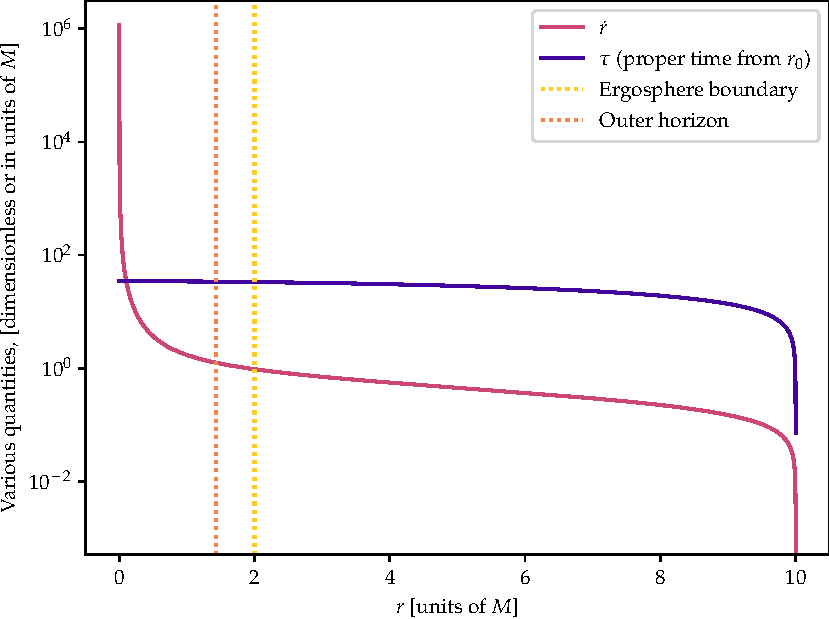
\includegraphics[width=.9\textwidth]{figures/kerr_infall}
\caption{EXPLAIN}
\label{fig:kerr_infall}
\end{figure}

\subsection{Exercise 6}

\subsubsection{Constant-$t$ hypersurfaces}

Three linearly independent vectors tangent to the \(t = \text{const}\) surface are \(\partial_r\), \(\partial_\theta \), \(\partial_\varphi \). 
They are orthogonal amongst themselves, since the only cross-terms in the metric are the \(g_{t \varphi }\) ones, but also because of that the \(\partial_\varphi \) vector is not orthogonal to \(\partial_t\): their product is %
\begin{align}
\partial_\varphi \cdot \partial_t = g_{t \varphi} \neq 0
\,.
\end{align}

This does not yet show that \(\partial_t\) is not hypersurface orthogonal: locally, we can find three vectors in the form \(\partial_r\), 
\(\partial_\theta \), \(v = \alpha \partial_t + \beta \partial_\varphi\) such that \(\partial_t\) is orthogonal to all of them. 
What should \(\alpha \) and \(\beta \) be? 
We are setting 
%
\begin{align}
0 &= v \cdot \partial_t \\
&= \alpha g_{tt} + \beta g_{t \varphi }  \\
- \beta g_{t \varphi } &= \alpha g_{tt}   \\
\frac{\beta }{\alpha} &= - \frac{ g_{t t }}{g_{t \varphi }}
\,.
\end{align}

The combination of metric coefficients appearing there is %
\begin{align}
\frac{g_{tt}}{g_{t \varphi }} &= 
\frac{- (1 - 2Mr / \rho^2)}{2Mar \sin^2 \theta / \rho^2} = \frac{2Mr - \rho^2}{2Mar \sin^2\theta } = \frac{2Mr - r^2 - a^2 \cos \theta }{2Mar \sin^2 \theta }  \\
\frac{\beta }{\alpha} &= \frac{ -2Mr + r^2 + a^2 \cos \theta}{2Mar \sin^2 \theta }
\,.
\end{align}

Locally, this works perfectly well; \(\partial_t\) not being hypersurface-orthogonal 
means that these surfaces cannot be extended to a global foliation of the spacetime. 

Let us set \(\theta = \pi /2\) for simplicity: then, 
%
\begin{align}
\frac{\beta }{\alpha} = \frac{r - 2M}{2Ma}
\,.
\end{align}

Now, we can see that at \(r = 2M\) (which is where the border of the ergosphere lies) this ratio approaches 0, therefore the 
solution must be \(\beta = 0\), or \(v = \alpha \partial_t\).

Any component along \(\partial_\varphi\) is not allowed at this boundary, although it is allowed at smaller and larger \(r\)s.
Also, the component along \(\varphi \) has an opposite sign above and below the ergosphere boundary. 

What this tells us is that the surfaces orthogonal to \(\partial_t\) cannot be extended through the ergosphere boundary.

\subsubsection{Killing vectors at infinity}

Let us show that the only Killing vectors which are timelike at \(r \to \infty \) are multiples of \(\partial_t\): if we take a linear combination \(v = \alpha \partial_t + \beta \partial_\varphi\), its norm will be 
%
\begin{align}
v^2 = \alpha^2 g_{tt} + 2 \alpha \beta g_{t \varphi } + \beta^2 g_{\varphi \varphi }
\,.
\end{align}

We want to ask that \(v^2 < 0\) in the \(r \to \infty \) limit: what constraint does this pose for \(\alpha \) and \(\beta \)? 

Well, as \(r \to \varphi \), the metric component \(g_{\varphi \varphi } \sim r^2 \), while \(g_{t \varphi } \sim 1 /r\) and \(g_{tt} \sim -1\).

Since \(\alpha\) and \(\beta\) are constants, the only way for \(v\) to be asymptotically timelike is if \(\beta = 0\) exactly, otherwise the \(\beta^2 g_{\varphi \varphi }\) term will mean \(v^2 \to + \infty \): therefore, \(v = \alpha \partial_t\) is a multiple of \(\partial_t\). 

\subsubsection{Timelike Killing vectors in the ergoregion}

We want to show that, given a point in the ergoregion \(r_+ < r < r_E\), it has a neighbourhood in which there is a timelike Killing vector.

This region is characterized by \(g_{tt} > 0\), while \(\Delta > 0\).
Also, \(g_{t \varphi } < 0\) and \(g_{\varphi \varphi } > 0\). 

This means that both the "regular" Killing vectors \(\partial_t\) and \(\partial_\varphi \) are spacelike. 

Can we make \(v = \alpha \partial_t + \beta \partial_\varphi \) timelike?
Its norm is 
%
\begin{align}
v^2 = g_{tt} \alpha^2 + 2 \alpha \beta g_{t \varphi } + \beta^2 g_{\varphi \varphi }
\,,
\end{align}
%
so we just need to show that there is a, possibly local, choice of \(\alpha \) and \(\beta \) such that \(v^2 < 0\).

Suppose it did not exist: so, at some coordinate point in the ergosphere, for all \(\alpha \) and \(\beta \), we would have \(v^2 \geq 0\). 
Then, consider an arbitrary vector \(u = \alpha \partial_t + \beta \partial_\varphi + \gamma \partial_r + \delta \partial_\theta \) at that point. 
Its norm will be  
%
\begin{align}
u^2 = \underbrace{\alpha^2 g_{tt} + 2 \alpha \beta g_{t \varphi } + \beta^2 g_{\varphi \varphi }}_{\geq 0} \underbrace{+ \gamma^2 g_{rr} + \delta^2 g_{\theta \theta }}_{\geq 0} \geq 0
\,.
\end{align}

Thus, we have shown that assuming this we can prove that all vectors in the ergosphere are either null or spacelike: 
this is impossible, since the metric can be always be cast into its diagonal, Minkowski 3+1 form by an appropriate local coordinate transformation.
Therefore, we must be able to make our Killing vector \(v\) timelike for some choice of \(\alpha \) and \(\beta \) everywhere.

In figure \ref{fig:kerr_killing} we show what this choice might actually look like.

\begin{figure}[ht]
\centering
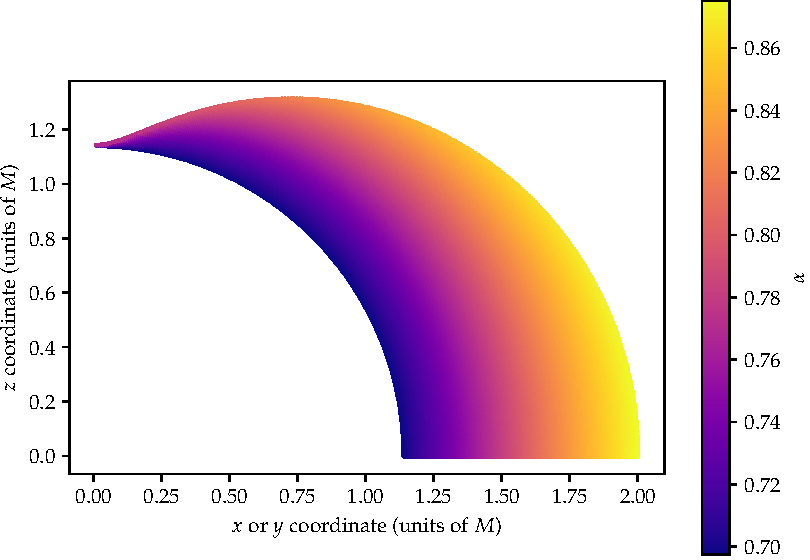
\includegraphics[width=\textwidth]{figures/kerr_killing}
\caption{Optimal value for \(\alpha \) as a function of position, for a BH with spin \(\chi = 0.99\). This is the value for \(\alpha \) which minimizes the norm of \(v\), assuming that \(\beta = 1 - \alpha \) (as well as \(M = 1\)); in all cases this minimum is negative.
Note that this is the locus of the minimum, but there is a range of acceptable values for \(\alpha \): this is why even at the ergosphere edge we don't have \(\alpha \to 1\). }
\label{fig:kerr_killing}
\end{figure}

\subsection{Exercise 7}

Hawking's area teorem states that the area of a BH can never increase; the area is related to the irreducible mass by 
%
\begin{align}
A \propto M _{\text{irr}}^2 = \frac{1}{2} M^2\left(1 + \sqrt{1 - \chi^2}\right)
\,,
\end{align}
%
where we are using \(c = G = 1\) units, as well as defining \(\chi = a / M = J / M^2\).  

We are taking two identical Kerr black holes with mass \(M\) and spin \(\chi\) and making them merge. 

We must then have %
\begin{align}
M_{\text{irr}}^{2, \text{ final}} &\geq 
M^{2, \text{ (1)}} _{\text{irr}}  +
M^{2, \text{ (2)}} _{\text{irr}}  
\\
M_f^2 \left( 1+ \sqrt{1 - \chi _f^2}\right) &\geq 2 M^2\left(1 + \sqrt{1 - \chi^2}\right)
\,,
\end{align}
%
where quantities labelled with an index \(f\) characterize the final BH. 

If the inital BHs were nonspinning, the equation states that %
\begin{align}
M_f^2 \left(1 + \sqrt{1 - \chi _f^2}\right) \geq 4 M^2
\,,
\end{align}
%
and we know that %
\begin{align}
M_f = 2M - E
\,,
\end{align}
%
where \(E\) is the energy lost by GW emission. 

This means we have a constraint on \(E\) and \(\chi _f\) as such: %
\begin{align}
\left(1 - \frac{E}{2M}\right)^2 \left(1 + \sqrt{1 - \chi _f^2}\right) \geq 1
\,.
\end{align}

If the black holes, instead, were initially spinning with \(\chi \neq 0\), the inequality becomes %
\begin{align}
\left(1 - \frac{E}{2M}\right)^2 \left(1 + \sqrt{1 - \chi _f^2}\right) \geq \frac{1 + \sqrt{1 - \chi^2}}{2}
\,,
\end{align}
%
which means that, if they were instead maximally spinning (\(\chi = 1\)) we will have 
%
\begin{align}
\left(1 - \frac{E}{2M}\right)^2 \left(1 + \sqrt{1 - \chi _f^2}\right) \geq \frac{1}{2}
\,.
\end{align}

The way to attain the maximum possible value for \(E\), in all these cases, is when \(\chi _f\) is as large as possible. 
A large \(\chi _f\) is indeed rather likely, since the product BH will be spinning due to the orbital angular momentum. 

If \(\chi _f = 1\), the general inequality reads: 
%
\begin{align}
\left(1 - \frac{E}{2M}\right)^2 \geq \frac{1 + \sqrt{1 - \chi^2}}{2} 
\,,
\end{align}
%
so in the \(\chi = 0\) case (nonspinning initial BHs, maximally spinning product) \emph{no} energy can be emitted; if the initial BHs are instead maximally spinning we have \(E \leq 2M ( 1 - 1/\sqrt{2}) \approx 0.59 M\).

Let us also look at a realistic situation: the best-fit values for the parameters of GW150914 are \(M_1 \approx 36M_{\odot}\), \(M_2 \approx 29M_{\odot}\); the initial spins are not well constrained but the effective spin parameter is \(\chi _{\text{eff}} \sim 0.05\), so let's assume the two BHs both had \(\chi = 0.05\). 

The final BH spin is quite large, \(\chi _f \sim 0.68\). 
Using all these, we can write the inequality: %
\begin{align}
(M_1 + M_2 - E)^2 \left(1 + \sqrt{1 - \chi_f^2}\right) &\geq (M_1^2 + M_2^2 ) \left(1 + \sqrt{1 - \chi^2}\right)  \\
(65 M_{\odot} - E)^2 \times 1.73 &\geq (49 M_{\odot})^2 \times 1.998  \\
E &\leq 65M_{\odot} - 49 M_{\odot} \sqrt{\frac{1.998}{1.73}} \approx 15 M_{\odot}
\,.
\end{align}

The best-fit value for the emitted energy, \(E \sim 3M_{\odot}\), estimated through other means, is well within this constraint.

A more complete analysis can actually give us a posterior distribution for the total variation in area \(\Delta A\); the posterior probability of \(\Delta A < 0\) can then be computed, with GW150814 this comes out to be \(< 5\%\) \cite{isiTestingBlackholeArea2021}.

\end{document}